\doublespacing
\chapter{System Implementation} \label{chap:sysImplementation}
%\version{v1.10.2015}

\doublespacing

The software and hardware requirement that was required to built our web application are following:\\
\section{Hardware Requirements}
Following are the hardware requirements of the proposed system:\\
•	Processors : Quad core system.\\
•	RAM : Minimum ram is 4GB.\\
•	HDD : At least 20GB.
\section{Software Requirements}
Following are the software requirements of the proposed system:
•	MS VSCode or MyEclipse : For front-end and back-end developments.\\
•	Postman : For testing the API’s before checking it by using HTTP requests.\\
•	SQL YOG : For database management.\\  
•	Browsers/clients like chrome for testing the output of the system design.
\newpage
\section{UI Implementation}
\subsection{Home Page}
When user visit in our web application he will enter to home page. The home page of our web application is shown in following Figure \ref{HPl}.All the information about bidding will be shown in home page. He can place bid only if he is login in our web application. In case of invalid URL in search. The Visitors  will be moved to 404 not found page which angular provide as wild card in routing and navigation listed at the last of routing.\\
\begin{figure}[h]
    \centering
    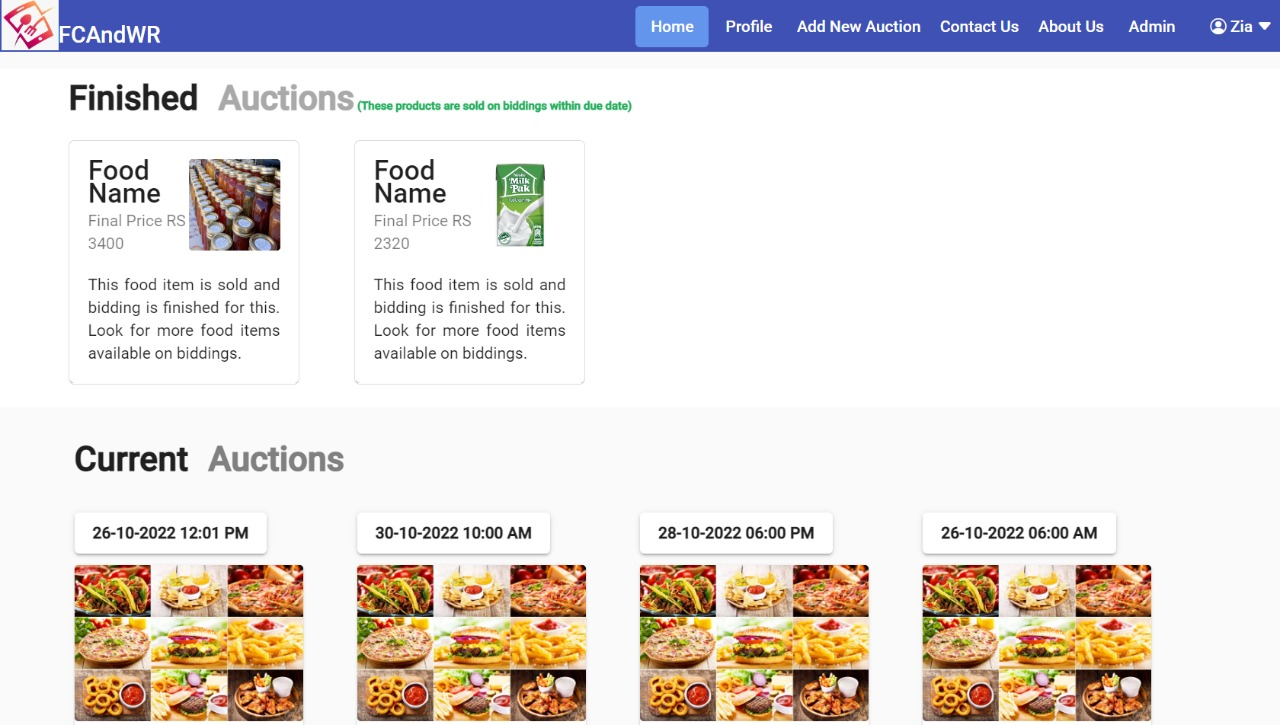
\includegraphics[width=15cm, height=15cm, keepaspectratio]{Homepage.jpeg}
    \caption{Home Page}
    \label{HPl}
\end{figure}

\subsection{Profile Page}
This page shows the user purchase history and user sales history. when a user won a bid he will be able to see his won bid in his profile section. The profile page of our web application is shown in following Figure \ref{pp}.
\begin{figure}[!h]
    \centering
    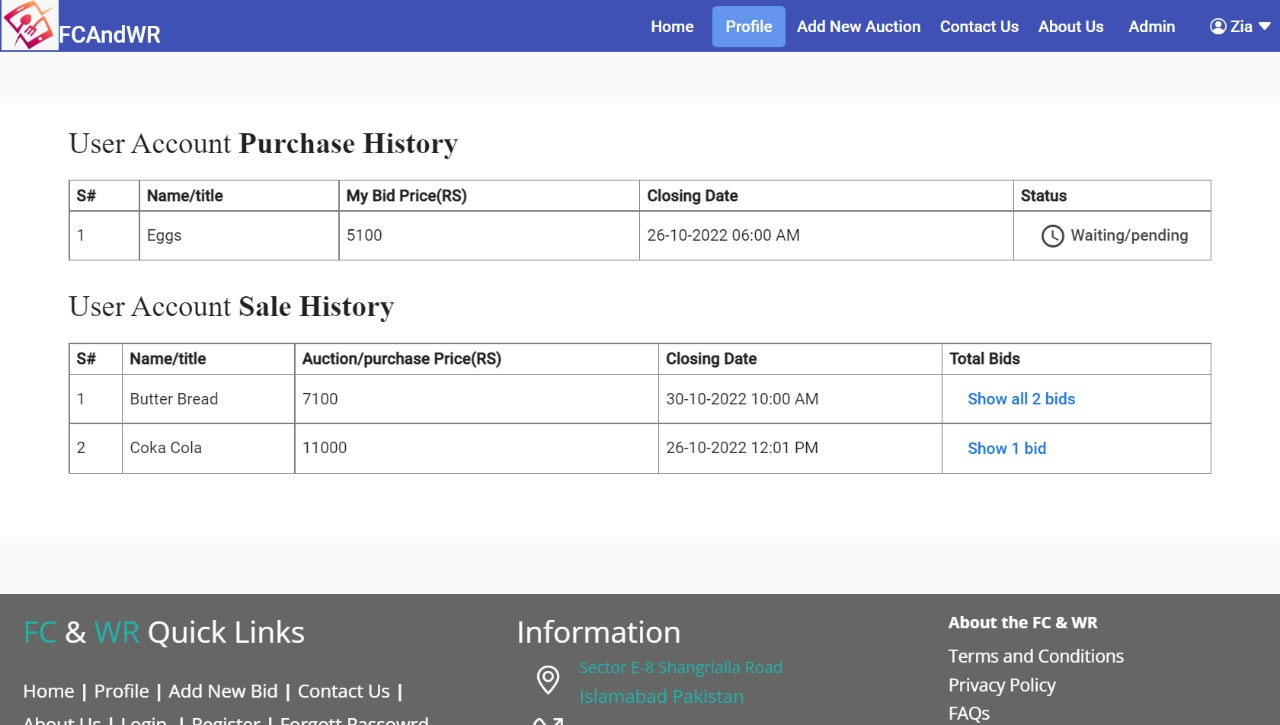
\includegraphics[width=15cm, height=15cm, keepaspectratio]{profile.jpeg}
    \caption{Profile Page}
    \label{pp}
\end{figure}
